\documentclass[12pt,letterpaper]{article}

\newenvironment{proof}{\noindent{\bf Proof:}}{\qed\bigskip}

\newtheorem{theorem}{Theorem}
\newtheorem{corollary}{Corollary}
\newtheorem{lemma}{Lemma} 
\newtheorem{claim}{Claim}
\newtheorem{fact}{Fact}
\newtheorem{definition}{Definition}
\newtheorem{assumption}{Assumption}
\newtheorem{observation}{Observation}
\newtheorem{example}{Example}
\newcommand{\qed}{\rule{7pt}{7pt}}

\newcommand{\assignment}[4]{
\thispagestyle{plain} 
\newpage
\setcounter{page}{1}
\noindent
\begin{center}
\framebox{ \vbox{ \hbox to 6.28in
{\bf CS446: Machine Learning \hfill #1}
\vspace{4mm}
\hbox to 6.28in
{\hspace{2.5in}\large\mbox{Problem Set #2}}
\vspace{4mm}
\hbox to 6.28in
{{\it Handed Out: #3 \hfill Due: #4}}
}}
\end{center}
}

\newcommand{\solution}[4]{
\thispagestyle{plain} 
\newpage
\setcounter{page}{1}
\noindent
\begin{center}
\framebox{ \vbox{ \hbox to 6.28in
{\bf CS446: Machine Learning \hfill #4}
\vspace{4mm}
\hbox to 6.28in
{\hspace{2.5in}\large\mbox{Problem Set #3}}
\vspace{4mm}
\hbox to 6.28in
{#1 \hfill {\it Handed In: #2}}
}}
\end{center}
\markright{#1}
}

\newenvironment{algorithm}
{\begin{center}
\begin{tabular}{|l|}
\hline
\begin{minipage}{1in}
\begin{tabbing}
\quad\=\qquad\=\qquad\=\qquad\=\qquad\=\qquad\=\qquad\=\kill}
{\end{tabbing}
\end{minipage} \\
\hline
\end{tabular}
\end{center}}

\def\Comment#1{\textsf{\textsl{$\langle\!\langle$#1\/$\rangle\!\rangle$}}}



\usepackage{graphicx,amssymb,amsmath, listings}
\lstset{language = Matlab}
\lstset{breaklines}
\lstset{extendedchars=false}

\oddsidemargin 0in
\evensidemargin 0in
\textwidth 6.5in
\topmargin -0.5in
\textheight 9.0in

\begin{document}

\solution{Jifu Zhao}{September $14$ $2015$}{1}{Fall 2015}
% Fill in the above, for example, as follows:
% \solution{Joe Smith}{\today}{1}{Fall 2012}

\pagestyle{myheadings}  % Leave this command alone

\begin{enumerate}
\item {\bf Answer to problem 1}

\begin{enumerate}
\item[{\bf a.}] {\bf Algorithm}\\

Suppose that we have {\bf m} training samples and there is {\bf n} variables.
And also, suppose that:
\begin{displaymath}
(x_1 = 1 \wedge x_5 = 0 \wedge x_7 = 1) \; \equiv \; (x_1 \wedge \neg x_5 \wedge x_7)
\end{displaymath}
\rule{400pt}{2pt}\\
{\bf Algorithm:} Finding accurate conjunctions\\
\rule{400pt}{1pt}
\begin{enumerate}

\item[1:] {\bf temp} := $x_1 \wedge \neg x_1 \wedge x_2 \wedge \neg x_2 \wedge......\wedge x_{n-1} \wedge \neg x_{n-1} \wedge x_n \wedge \neg x_n$

\item[2:] {\bf for} i := 1:m\\
\indent \qquad {\bf if} $instance(i)$ is positive(+) {\bf then}\\
\indent \qquad \qquad {\bf remove} any item in temp that is inconsistent with $instance(i)$\\
\indent \qquad \qquad (for example, if in $instance(i)$, $x_j = 1$, then remove $\neg x_j$ from temp,\\
\indent \qquad \qquad else if $x_j = 0$, then remove $x_j$)\\
\indent \qquad {\bf end if}\\
{\bf end for}

\item[3:] {\bf for} i := 1:n\\
\indent \qquad {\bf check} if there is $x_i \wedge \neg x_i$ exists\\
\indent \qquad {\bf if} exists\\
\indent \qquad \qquad {\bf remove} both $x_i$ and $\neg x_i$ from temp\\
\indent \qquad {\bf end if}\\
{\bf end for}

\item[4:] {\bf for} i := 1:m\\
\indent \qquad {\bf check} whether temp is consistent with $instance(i)$\\
\indent \qquad {\bf if} inconsistent\\
\indent \qquad \qquad {\bf return:} Not found\\
\indent \qquad \qquad {\bf stop}\\
\indent \qquad {\bf end if}\\
{\bf end for}
\end{enumerate}
\rule{400pt}{2pt}\\

{\bf Algorithm Explanation}:\\

According to {\bf Find-S Algorithm} (Tom Mitchell, $Machine learning$, 1997), in the proposed algorithm, we first generate the most specific condition: $x_1 \wedge \neg x_1 \wedge x_2 \wedge \neg x_2 \wedge......\wedge x_{n-1} \wedge \neg x_{n-1} \wedge x_n \wedge \neg x_n$, which is assigned to {\bf temp}. Then, in {\bf step 2}, compare this most specific case with the instances whose label is positive(+). In this procedure, we will remove any sub-term from {\bf temp} that is inconsistent with the $instance(i)$. So, after step 2, in {\bf temp}, only those that are consistent with all training samples will be left. In {\bf step 3}, we consider the situation that both $x_i$ and $\neg x_i$ appear simultaneous in {\bf temp}, then remove them from {\bf temp}. Finally, in {\bf step 4}, we compare the {\bf temp} with all samples to make sure that our final conclusion is right.\\

\item[\bf{b.}] {\bf Proof}\\
\begin{enumerate}
\item[1: ] In {\bf step 4}, through comparing the proposed conjunction with all instances, we can make sure that if there is one conjunction generated through our algorithm, it will be consistent with all instances.
\item[2: ] In more details, through {\bf step 2} and {\bf step 3}, we can make sure that the remaining temp will only keep the term that is consistent with all positive(+) instances.
\item[3: ] Through {\bf step 4}, we can make sure that our algorithm will be consistent with all negative(-) instances. Or there will be no result generated.\\

So, in conclusion, if there is one conjunction generated as the result, it will be consistent will all training samples.\\
\end{enumerate}

\item[\bf{c.}] {\bf Complexity analysis}\\
\begin{enumerate}
\item[1: ] In {\bf step 2}, there will be {\bf m} iteration. And in every iteration, we need to maximumly compare {\bf n} terms, so the maximum comparison will be $m*n$.
\item[2: ]In {\bf step 3}, we will do the check for maximumly {\bf n} times. So the maximum procedure will be $n$.
\item[3: ]In {\bf step 4}, there will be maximumly {\bf m} procedure. So the maximum complexity will be $m$.
\item[4: ]So, in conclusion, the final complexity will be $m*n+m+n$. It can also be represented by $O(mn)$.\\
\end{enumerate}

\item[\bf{d.}] {\bf Ability analysis}\\

\begin{enumerate}
\item[1: ] If the label got from the algorithm is {\bf positive(+)}, it means that the correct label for this new example will be positive(+). The reason is clear. In our algorithm, all terms that is inconsistent with all the training examples will be removed. If we have more information, we will only remove more terms from our final conjunction. But this will not affect the fact that the label for new example is positive(+). So, no matter how much more information is included, the label for new example will always be positive(+).\\

\item[2: ] If the label for the new example is {\bf negative(-)}, we cannot determine whether or not its real label is negative(-) or positive(+). The reason is also clear. When the label for the new example is negative(-), if we have more information, we will remove more terms from the conjunction we got. So, after removal, it is possible that we can get a positive(+) label for the new example. So, if the label for the new example is negative(-), we cannot determine easily. We need more information to get a more reliable conclusion.\\
\end{enumerate}
\end{enumerate}

\item {\bf Answer to problem 2}

\begin{enumerate}
\item[{\bf a.}] {\bf Derivation\\}

In algebra, the hyperplane $\vec{w}^T \vec{x} + \theta = 0$ means that the vector $\vec{w}$ is perpendicular to the hyperplane, and the $\theta$ means the shift from the hyperplane that goes across the zero point. So, in order to calculate the distance between the point $\vec{x_0}$ and the hyperplane $\vec{w}^T \vec{x} + \theta = 0$, we first find one point on the hyperplane, which is $\vec{x}$, the vector formed by $\vec{x}$ and $\vec{x_0}$ will be $\vec{x_0}-\vec{x}$. Next, we only need to calculate the projection of $\vec{x_0}-\vec{x}$ on $\vec{w}$. It is defined as $\frac{|\vec{w}^T(\vec{x_0}-\vec{x})|}{||\vec{w}||}$. Since $\vec{w}^T \vec{x} + \theta = 0$, so $\vec{w}^T \vec{x} = - \theta$. So $\frac{|\vec{w}^T(\vec{x_0}-\vec{x})|}{||\vec{w}||}$ will change into $\frac{|\vec{w}^T \vec{x_0} + \theta|}{||\vec{w}||}$. So the distance between $\vec{x_0}$ and the hyperplane $\vec{w}^T \vec{x} + \theta = 0$ is:
\begin{displaymath}
d = \frac{|\vec{w}^T \vec{x_0} + \theta|}{||\vec{w}||}
\end{displaymath}

\item[{\bf b.}] {\bf Distance between two hyper-planes}\\

The two hyperplanes, $\vec{w}^T \vec{x} + \theta_1 = 0$ and $\vec{w}^T \vec{x} + \theta_2 = 0$. They are parallel since they have the same $\vec{w}^T$. To calculate the distance between these two hyperplanes, we only need to find two point from each of these two hyperplanes, and calculate the projection of the vector formed by these two points on $\vec{w}$. Suppose we choose $\vec(x_1)$ from the first hyperplane, so $\vec{w}^T \vec{x_1} + \theta_1 = 0$. And choose $\vec(x_2)$ from the first hyperplane, so $\vec{w}^T \vec{x_2} + \theta_2 = 0$. The vector formed by $\vec(x_1)$ and $\vec(x_2)$ will be $\vec(x_1 - x_2)$. So the projection of $\vec(x_1 - x_2)$ on $\vec{w}$ will be $\frac{|\vec{w}^T(\vec{x_1}-\vec{x_2})|}{||\vec{w}||}$. Since $\vec{w}^T \vec{x_1} + \theta_1 = 0$ and $\vec{w}^T \vec{x_2} + \theta_2 = 0$, so $\vec{w}^T \vec{x_1} = - \theta_1$ and $\vec{w}^T \vec{x_2} = - \theta_2$. So the distance between these two hyperplanes will be:
\begin{displaymath}
d = \frac{|\theta_1 - \theta_2|}{||\vec{w}||}
\end{displaymath}
\end{enumerate}

\item {\bf Answer to problem 3}

\begin{enumerate}
\item[{\bf a.}] {\bf Linear separability}\\

\begin{enumerate}

\item[{\bf a.1 }] {\bf Linear separability}\\

{\bf 1, First, prove that if $D$ is linearly separable, then there exists a hyperplane that satisfies condition (3) with $\delta = 0$.}\\

If $D$ is linearly separable, then according to the definition, 
\begin{equation}
\label{eq:separable}
y_i = \begin{cases}
 1 & \mbox{if } \vec{w}^T \vec{x_i} + \theta \ge 0 \\
-1 & \mbox{if } \vec{w}^T \vec{x_i} + \theta < 0. \\
\end{cases}
\end{equation}

For the case that $\vec{w}^T \vec{x_i} + \theta \ge 0$, we can find an example $\vec{x_m}$ that is $closest$ to the hyperplane among all positive examples. Set it to be $\vec{w}^T \vec{x_m} + \theta = A \ge 0$. Also, for the cases of $\vec{w}^T \vec{x_j} + \theta < 0$, we can also find a negative example $\vec{x_n}$ that is closest to the hyperplane among negative examples. Set it to be $\vec{w}^T \vec{x_n} + \theta = B < 0$. So, we have $A \ge 0 > B$.\\

Now, let's define $\alpha$ that satisfy $A-\alpha \ge 0 > B - \alpha$. So, now we have $\vec{w}^T \vec{x_i} + \theta -\alpha = A - \alpha \ge 0 $ and $\vec{w}^T \vec{x_n} + \theta - \alpha = B - \alpha < 0$.\\

More specifically, let's find an $\alpha$ that makes the hyperplane $\vec{w}^T \vec{x} + \theta - \alpha = 0$ have the same distance for $\vec{x-m}$ and $\vec{x-n}$. So, we have
\begin{center}
$\frac{|\vec{w}^T \vec{x_m} + \theta - \alpha|}{||\vec{w}||} = \frac{|\vec{w}^T \vec{x_n} + \theta - \alpha|}{||\vec{w}||}$.
\end{center}

So, we can get that $|\vec{w}^T \vec{x_m} + \theta - \alpha| = |\vec{w}^T \vec{x_n} + \theta - \alpha|$, then we have $\vec{w}^T \vec{x_m} + \theta - \alpha = -(\vec{w}^T \vec{x_n} + \theta - \alpha)$, which means that $ A - \alpha = - B + \alpha$. So, $ \alpha = \frac{A + B}{2}$. So, the hyperplane $\vec{w}^T \vec{x} + \theta - \alpha = 0$ will separate the set $D$. \\

So, when we choose $\vec{x_m}$ and $\vec{x_n}$, we have $\vec{w}^T \vec{x_m} + \theta - \alpha = \frac{A - B}{2} \ge 0$ and we also have $\vec{w}^T \vec{x_n} + \theta - \alpha = -\frac{A - B}{2} < 0$. If we multiply $\beta = \frac{2}{A - B}$ on both side, we can get $\beta \cdot \vec{w}^T \vec{x_m} + \frac{\theta - \alpha}{\beta} = 1$ and $\beta \cdot \vec{w}^T \vec{x_n} + \frac{\theta - \alpha}{\beta} = -1$.\\ 

Now, let $ \vec{w'}^T = \beta \cdot \vec{w}^T$, and $\theta' = \frac{\theta - \alpha}{\beta}$, we will have that $y_i(\vec{w'}^T \vec{x_i} + \theta') = 1 - \delta$ to separate the set $D$, and $\delta = 0$.\\

So, from condition (1), we can get condition (3).\\

{\bf 2, Secondly, let's prove that from (3), we can get (1).\\}

From condition (3) $y_i(\vec{w}^T \vec{x_i} + \theta) \geq 1 - \delta$, when $\delta = 0$, we will have $y_i(\vec{w}^T \vec{x_i} + \theta) \geq 1$. It is very obvious that when $\vec{w}^T \vec{x_i} + \theta \geq 1$, we will have $\vec{w}^T \vec{x_i} + \theta \geq 0$. And when $\vec{w}^T \vec{x_i} + \theta < -1$, we will have $\vec{w}^T \vec{x_j} + \theta < 0$.\\

So, from condition(3), we can easily prove the correctness of condition(1).\\

{\bf In conclusion}, the data set $D$ is linearly separable if and only if there exists a hyperplane that satisfies condition(3) with $\delta = 0$.\\

{\bf 3, If there exists a hyperplane that satisfies condition(3) with $\delta > 0$, our conclusion will be determined by the value of $\delta$.}\\

If $\delta < 1$, we can conclude that $y_i(\vec{w}^T \vec{x_i} + \theta) > 0$, which is consistent with the condition(1). So, {\bf when $0 < \delta < 1$, we can conclude that the set $D$ is separable}.\\

But when $\delta \ge 1$, we will have $y_i(\vec{w}^T \vec{x_i} + \theta) \ge 1-\delta$. However, we can only know that $1-\delta \le 0$, we cannot determine whether or not $y_i(\vec{w}^T \vec{x_i} + \theta) > 0$. So, {\bf when $\delta \ge 1$, we cannot determine whether or not the set $D$ is separable}.\\

\item[{\bf a.2 }] {\bf Trivial optimal solution}\\

When $y_i(\vec{w}^T \vec{x_i} + \theta) \ge -\delta$, if $\delta \ge 0$, the optimal solution for $\delta$ will be $\delta = 0$. When $\delta = 0$, we will have $y_i(\vec{w}^T \vec{x_i} + \theta) \ge 0$, so the optimal solution for this will be:
$ \vec{w} = \vec{0}$ and $\theta = 0$. This solution have no meaning for this question.\\

So, if we use the format that $y_i(\vec{w}^T \vec{x_i} + \theta) \ge -\delta$, we can only get the optimal solution that $\delta = 0$, $ \vec{w} = \vec{0}$ and $\theta = 0$, which have no meaning for us. But if we choose the format in (2) to (4), our optimal solution will not be $ \vec{w} = \vec{0}$ and $\theta = 0$. So, (2) to (4) will help us actually solve this problem.\\

\item[{\bf a.3 }] {\bf Optimal solutions}\\

When $\vec{x_1}^T = \begin{bmatrix} 1 & 1 & \ldots & 1 \end{bmatrix}$, $\vec{x_2}^T = \begin{bmatrix} -1 & -1 & \ldots & -1 \end{bmatrix}$ and $y_1 = 1$, $y_2 = -1$. Apply (3) to $\vec{x_1}$, $\vec{x_2}$, $y_1$ and $y_2$. We can get that $w_1 + w_2+ \ldots w_n + \theta \ge 1 - \delta$ and  $w_1 + w_2 + \ldots w_n - \theta \ge 1 - \delta$. Considering the condition that $\delta = 0$, we will have that $w_1 + w_2 + \ldots w_n \ge 1 - \theta$ and $w_1 + w_2 + \ldots w_n \ge 1 + \theta$.\\

So, the final conclusion will be: $w_1 + w_2 + \ldots w_n \ge 1 - |\theta|$.\\
\end{enumerate}

\item[{\bf b.}] {\bf Linear Programming}\\

\begin{enumerate}
\item[{\bf b.1 }] {\bf Rewrite the linear program}\\

from (2) to (4), we can get 
\begin{eqnarray}
    \min_{\delta, \vec{w}, \theta} & & \delta \\
    \textrm{subject to } & & y_i \vec{w}^T \vec{x_i} + y_i \theta \geq 1 - \delta \\
    \delta \geq 0
\end{eqnarray}

\begin{eqnarray}
    \min_{\delta, \vec{w}, \theta} & & \delta \\
    \textrm{subject to } & & y_i \vec{w}^T \vec{x_i} + y_i \theta  + \delta \geq 1 \\
    \delta \geq 0
\end{eqnarray}

Write (5) to (7) into matrix, we can get:\\
\begin{eqnarray}
    & & z(\vec{t}) = \delta = \begin{bmatrix}
     0 & 0 & 1 
     \end{bmatrix} * \begin{bmatrix}
    \vec{w} \\ \theta \\ \delta 
    \end{bmatrix}\\    
    \textrm{subject to } & & \begin{bmatrix}
    y_1\vec{x_1}^T & y_1 & 1 \\
    y_2\vec{x_2}^T & y_2 & 1 \\
    \ldots & \ldots & \ldots \\
    y_m\vec{x_m}^T & y_m & 1 \\
    0 & 0 & 1 \\    
    \end{bmatrix} * \begin{bmatrix}
    \vec{w} \\ \theta \\ \delta
    \end{bmatrix} \geq \begin{bmatrix}
    1 \\ 1 \\ \ldots \\ 1 \\ 0
    \end{bmatrix}
\end{eqnarray}\\

So, choose $\vec{c}^T = \begin{bmatrix} 0 & 0 & 1 \end{bmatrix}$, $\vec{t} = \begin{bmatrix} \vec{w} \\ \theta \\ \delta \end{bmatrix}$, $A = \begin{bmatrix}
    y_1\vec{x_1}^T & y_1 & 1 \\
    y_2\vec{x_2}^T & y_2 & 1 \\
    \ldots & \ldots & \ldots \\
    y_m\vec{x_m}^T & y_m & 1 \\
    0 & 0 & 1 \\    
    \end{bmatrix}$
    and $b = \begin{bmatrix} 1 \\ 1 \\ \ldots \\ 1 \\ 0 \end{bmatrix}$.\\ 
    
So, the question turns to be a linear question, which is 
\begin{eqnarray*}
  & & z(\vec{t}) = \vec{c}~^T \vec{t} \\
\textrm{subject to} & & A \vec{t} \geq \vec{b}
\end{eqnarray*}

We can solve this problem through linear programming.\\

The Matlab code for {\bf findLinearDiscriminant.m} is shown as follows.\\
\rule{400pt}{2pt}
\begin{lstlisting}
function [w,theta,delta] = findLinearDiscriminant(data)
%% setup linear program
[m, np1] = size(data);
n = np1-1;

% write your code here

A = zeros(m+1, n+2);
for j = 1:m
    A(j, 1:n) = data(j, n+1).*data(j, 1:n);
    A(j, n+1) = data(j, n+1);
    A(j, n+2) = 1;
end
A(m+1, n+2) = 1;

b = zeros(m+1, 1);
b(1:m, 1) = 1;

c = zeros(n+2, 1);
c(n+2, 1) = 1;

%% solve the linear program
%adjust for matlab input: A*x <= b
[t, z] = linprog(c, -A, -b);

%% obtain w,theta,delta from t vector
w = t(1:n);
theta = t(n+1);
delta = t(n+2);

end
\end{lstlisting}
\rule{400pt}{2pt}\\

\item[{\bf b.2 }] {\bf Learning Conjunctions as an LP}\\

The manually generated data set in {\bf hw1sample2d.txt} is as follows:\\
\begin{center}
$\begin{matrix}
1 & 1 &  1 \\ 1 & 0 & -1 \\ 0 & 1 & -1 \\ 0 & 0 & -1\\
\end{matrix}$\\
\end{center}


The Matlab code for {\bf plot2dSeparator.m} is shown as follows.\\

\rule{400pt}{2pt}
\begin{lstlisting}
function plot2dSeparator(w, theta)

n = length(w);
if n ~= 2
    disp('only 2d data supported.')
else
    x = -0.1:0.01:1.1;
    y = -w(1) * x / w(2) - theta / w(2);
    plot(x, y, 'LineWidth',2);
end

\end{lstlisting}
\rule{400pt}{2pt}\\

The output of {\bf plot2dSeparator.m} and {\bf plot2dData.m} is shown in figure 1. The red points means the label is positive(+) and the green points means that the label is negative(-). The blue line successfully separate those two labels data.\\

\begin{figure}[h]
\centering
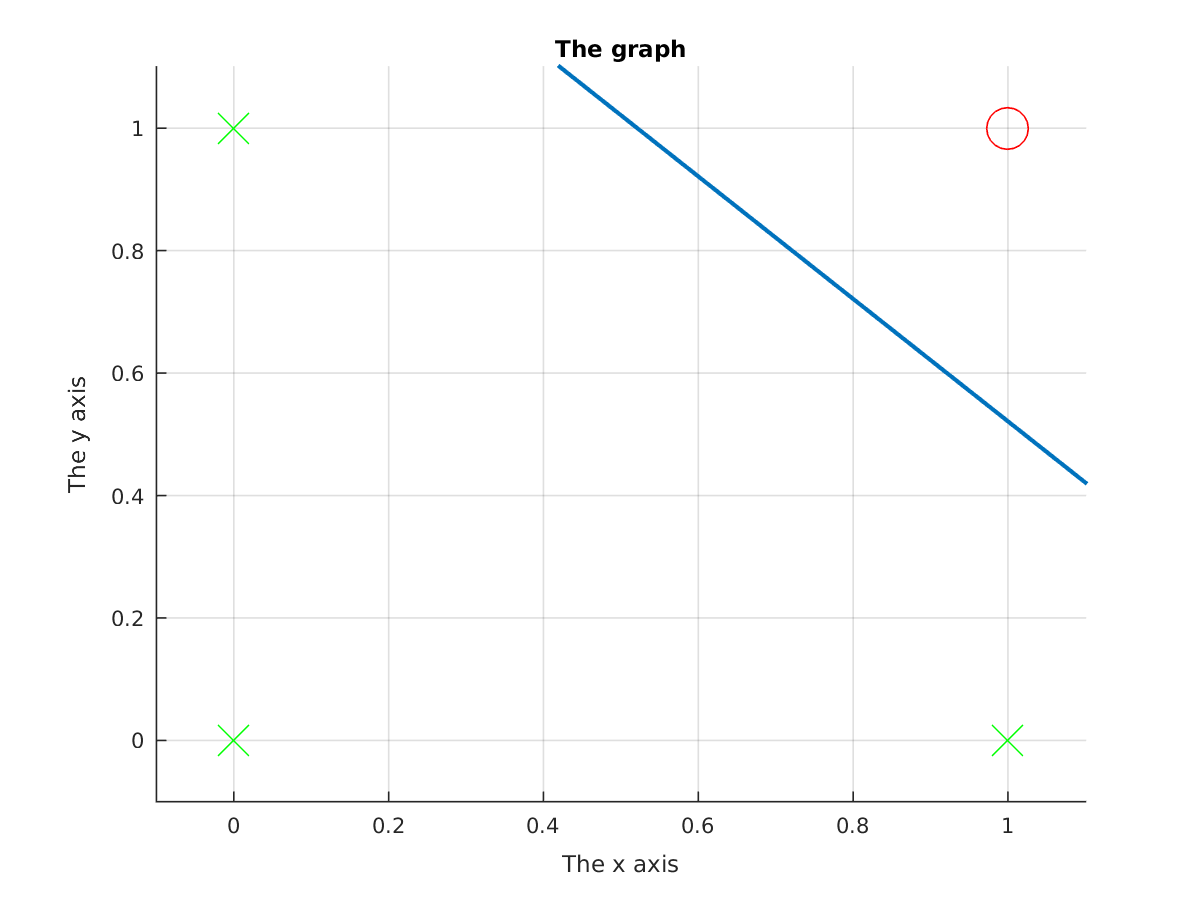
\includegraphics[height = 350pt]{2d.png}
\caption{2D data and separator}
\end{figure}

The output for {\bf hw1conjunction.txt} are show below:\\

\rule{400pt}{2pt}
\begin{center}
$\begin{bmatrix}
w_1 \\ w2 \\ w_3 \\ w_4 \\ w_5 \\ w_6 \\ w_7 \\ w_8 \\ w_9 \\ w_{10} \\ 
\end{bmatrix}$ = $\begin{bmatrix}
2.910374 \\ -2.049762 \\ 0.177469 \\ 190.519580 \\ 0.139878 \\ -3.100985 \\ -2.953437 \\ -193.277767 \\ 1.167917 \\ -8.894156 \\
\end{bmatrix}$\\

\end{center}


And the corresponding $\theta$ and $\delta$ are: \\
\begin{center}
$\theta = -90.211531$ and $\delta = -0.000000$\\
\end{center}
\rule{400pt}{2pt}\\

And the expression for final discriminant function are:\\
\begin{center}
$\vec{w}^T \vec{x} - 90.211531 = 1$
\end{center}
Which can be written as:\\
\begin{center}
$\vec{w}^T \vec{x} - 91.211531 = 0$
\end{center}

Corresponding to the output, we can get the expression for the conjunction:\\

\begin{center}
$\vec{x_4} \wedge \neg \vec{x_8}$ \\
\end{center}

The value of $\delta$ is very close to 0, which is consistent with our previous theory. This means that the data set can be linearly separated.\\

\item[{\bf b.3 }] {\bf Learning Badges}\\

The Matlab code for {\bf computeLabel.m} is shown as follows. \\

\rule{400pt}{2pt}
\begin{lstlisting}
function y = computeLabel(x, w, theta)

y0 = w' * x + theta;

if y0 >= 0
    y = 1;
else
    y = -1;
end

end

\end{lstlisting}
\rule{400pt}{2pt}\\

Based on this code, run the learnBadges.m, we can get the result shown in figure 2.\\
\begin{figure}[h]
\centering
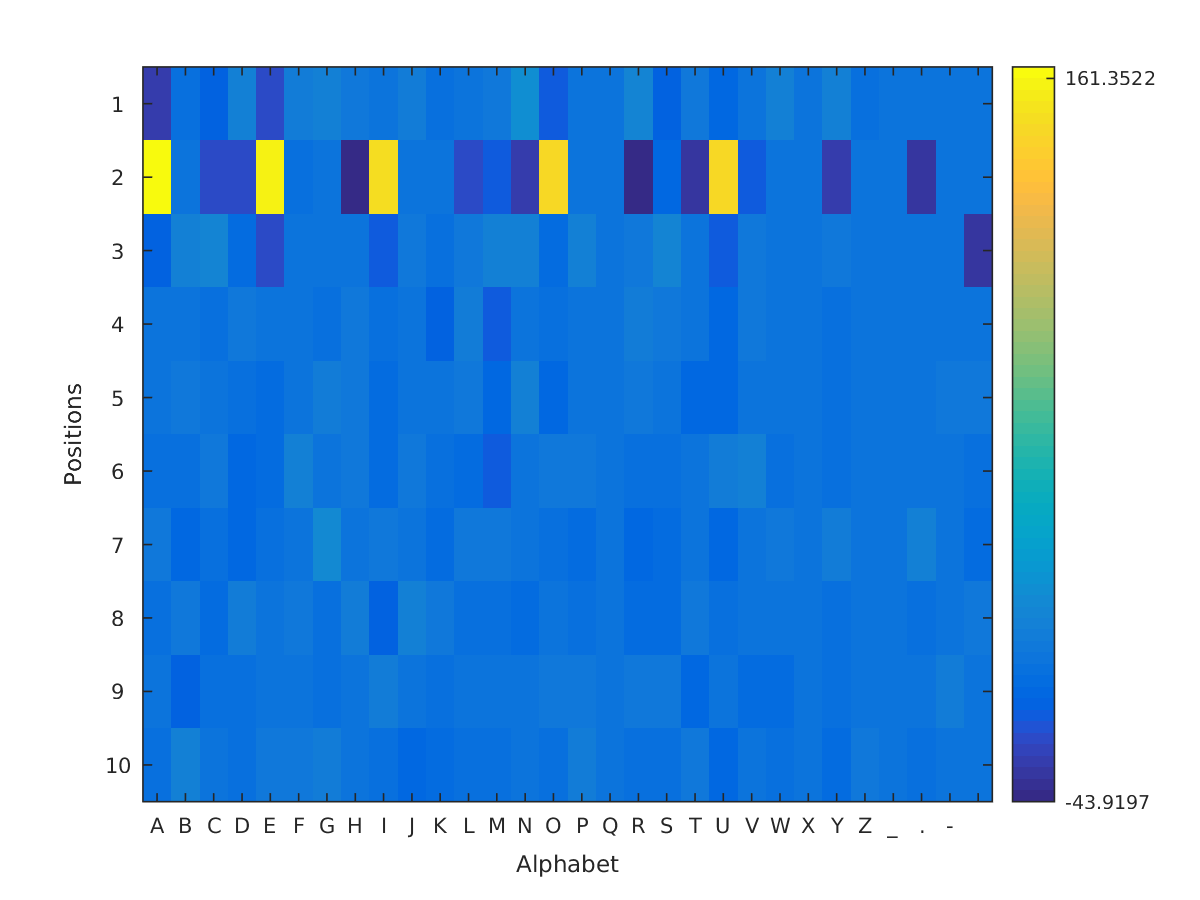
\includegraphics[height = 350pt]{badges.png}
\caption{Result for Badges game 1}
\end{figure}

The corresponding value are:\\
\begin{center}
$\delta = 1.2612e-19$\\
$accuracyInTrain = 1$\\
$accuracyInTest = 1$\\
\end{center}

Now, change the value for {\bf alphabet} and {\bf positions} to get other results. After some changes, I find that when:\\
\begin{center}
$alphabet = 'ABCDEFGHIJKLMNOPQRSTU'$\\
$positions = 3:10$\\
\end{center} 

The output will be:\\
\begin{center}
$\delta = 2.2524e-11$\\
$accuracyInTrain = 1$\\
$accuracyInTest = 0.7234$\\
\end{center}

And the corresponding figure is shown in figure 3.\\
\begin{figure}[h]
\centering
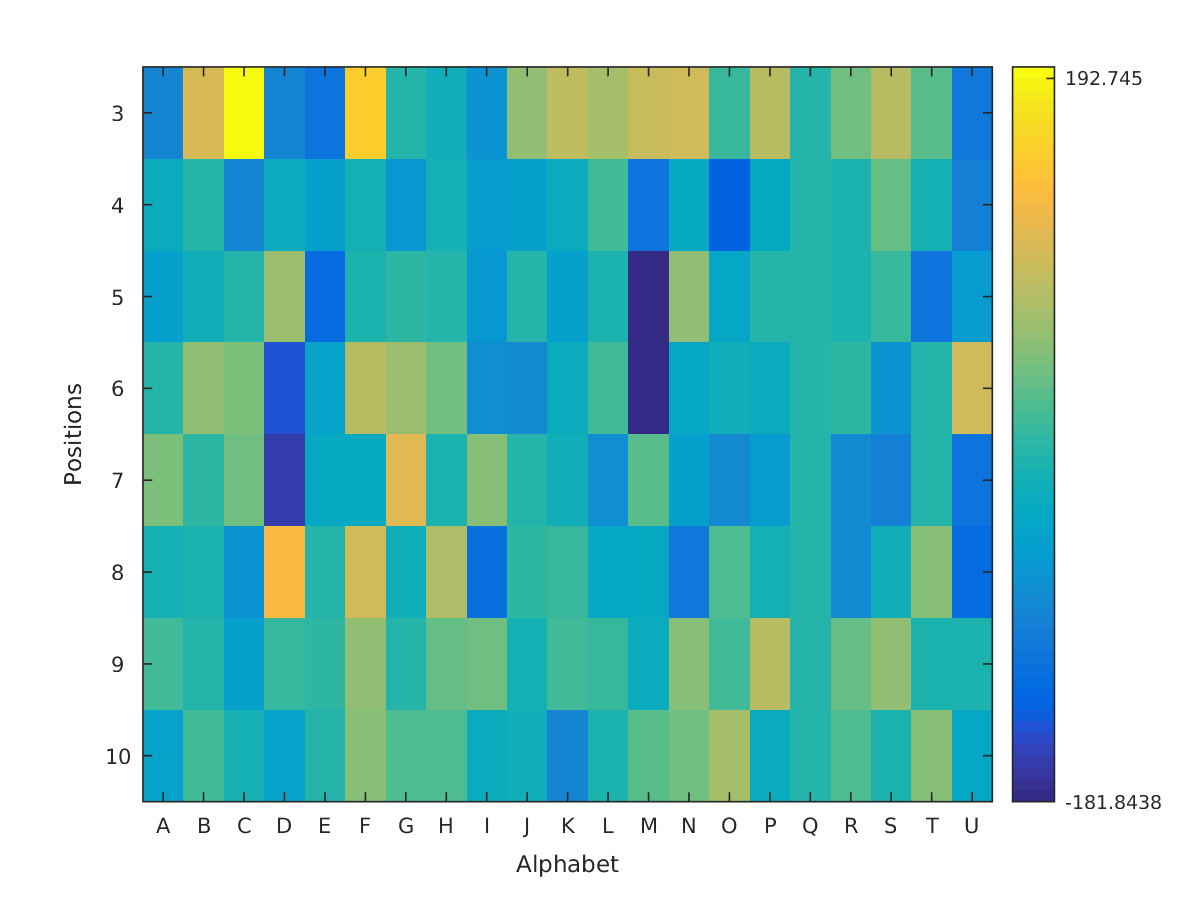
\includegraphics[height = 350pt]{badges2.png}
\caption{Result for Badges game 2}
\end{figure}

Compared with figure 2, it is easy to find that in figure 3, the relation of alphabet and position is not very clear. But in figure 2, the relation of alphabet and position is very clear.\\

\item[{\bf b.4 }] {\bf Learning Multiple Hyperplanes}\\

When $\vec{w}$ is known, the question can be simplified.\\

from (2) to (4), we can get 
\begin{eqnarray}
    \min_{\delta, \vec{w}, \theta} & & \delta \\
    \textrm{subject to } & & y_i \theta  + \delta \geq 1 - y_i \vec{w}^T  \vec{x_i}\\
    \delta \geq 0
\end{eqnarray}

Write (10) to (12) into matrix, we can get:\\
\begin{eqnarray}
    & & z(\vec{t}) = \delta = \begin{bmatrix}
     0 & 1 
     \end{bmatrix} * \begin{bmatrix}
    \theta \\ \delta 
    \end{bmatrix}\\    
    \textrm{subject to } & & \begin{bmatrix}
    y_1 & 1 \\
    y_2 & 1 \\
    \ldots & \ldots \\
    y_m & 1 \\
    0 & 1 \\
    \end{bmatrix} * \begin{bmatrix}
    \theta \\ \delta
    \end{bmatrix} \geq \begin{bmatrix}
    1 - y_1 \vec{w}^t \vec{x_1} \\ 1 - y_1 \vec{w}^t \vec{x_2} \\ \ldots \\ 1 - y_1 \vec{w}^t \vec{x_m} \\ 0
    \end{bmatrix}
\end{eqnarray}\\

So, choose $\vec{c}^T = \begin{bmatrix} 0 & 1 \end{bmatrix}$, $\vec{t} = \begin{bmatrix} \theta \\ \delta \end{bmatrix}$, $A = \begin{bmatrix}
    y_1 & 1 \\
    y_2 & 1 \\
    \ldots & \ldots \\
    y_m & 1 \\  
    0 & 1 \\
    \end{bmatrix}$
    and $b = \begin{bmatrix}
    1 - y_1 \vec{w}^t \vec{x_1} \\ 1 - y_1 \vec{w}^t \vec{x_2} \\ \ldots \\ 1 - y_1 \vec{w}^t \vec{x_m} \\ 0
    \end{bmatrix}$.\\ 
    
So, the question turns to be a linear question, which is 
\begin{eqnarray*}
  & & z(\vec{t}) = \vec{c}~^T \vec{t} \\
\textrm{subject to} & & A \vec{t} \geq \vec{b}
\end{eqnarray*}

We can solve this problem through linear programming.\\

The Matlab code for {\bf findLinearThreshold.m} is shown below:\\

\rule{400pt}{2pt}
\begin{lstlisting}
function [theta,delta] = findLinearThreshold(data,w)
%% setup linear program
[m, np1] = size(data);
n = np1 - 1;

% write your code here

A = zeros(m+1 ,n);
A(1:m, 1) = data(1:m, np1);
A(m+1,1) = 0;
A(:, 2) = 1;

b = zeros(m+1, 1);
b(1:m, 1) = data(1:m, 1:n) * w;
for i = 1:m
    b(i) = 1 - data(i, np1) * b(i);
end
b(m+1, 1) = 0;

c = [0; 1];

%% solve the linear program
%adjust for matlab input: A*x <= b

[t, z] = linprog(c, -A, -b);

%% obtain w,theta,delta from t vector

theta = t(1);
delta = t(2);

end
\end{lstlisting}
\rule{400pt}{2pt}\\

The plots for different separators are shown in figure 4.\\

\begin{figure}[h]
\centering
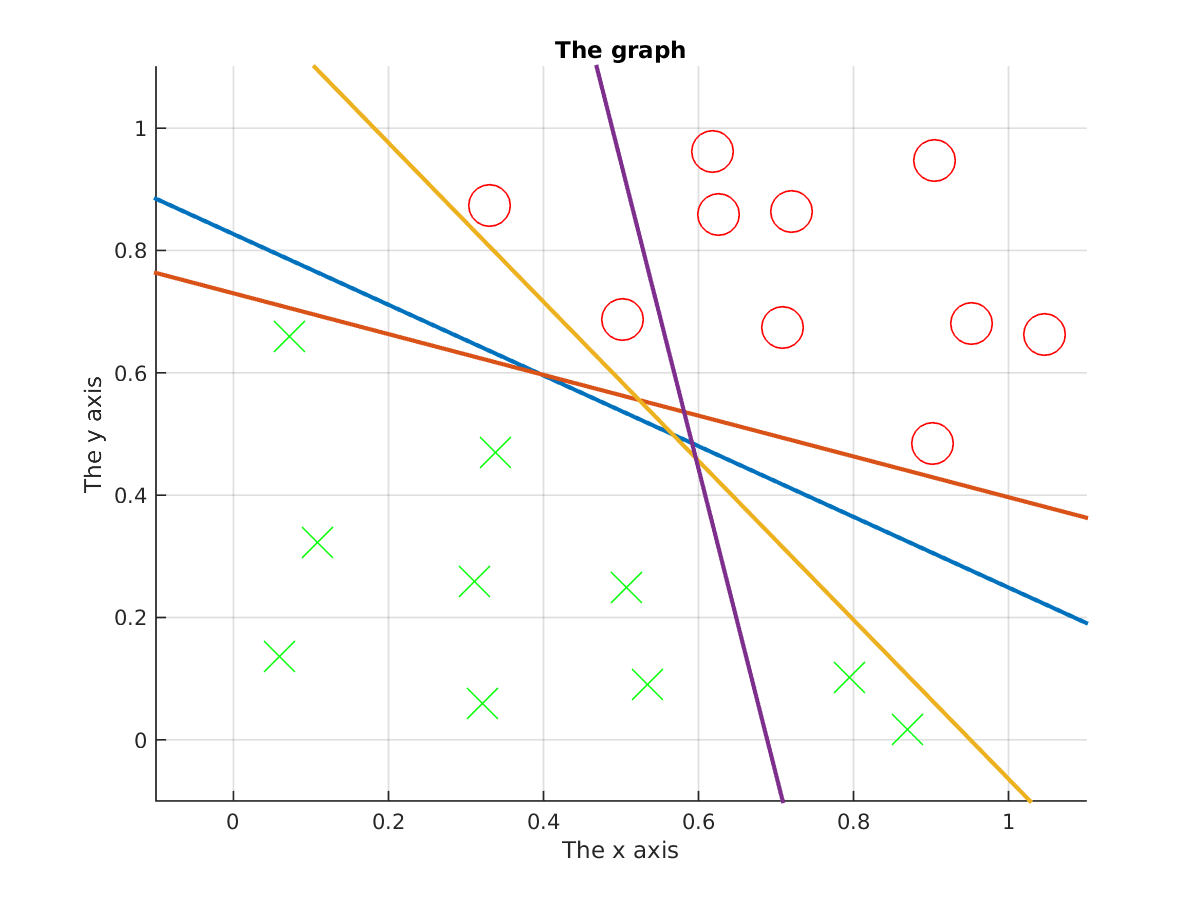
\includegraphics[height = 350pt]{multiple.png}
\caption{Multiple hyperplane separator}
\end{figure}

Through calculation, the weight is $\vec{w}^T = [170.009960, 294.223222]$ and the corresponding values are $\theta =-243.262997$ and $\delta = 0.000000$.\\

Using $\vec{w}^T = [100.0, 300.0]$, the corresponding values are $\theta = -218.994588$ and $\delta = 0.000000$.\\

Using $\vec{w}^T = [130.0, 100.0]$, the corresponding values are $\theta = -123.611614$ and $\delta = 0.000000$.\\

Using $\vec{w}^T = [500.0, 100.0]$, the corresponding values are $\theta =-344.335000$ and $\delta = 92.965000$.\\

Compared those 4 plots(on clockwise direction, the plots are 1, 2, 3, and 4), it is easy to find that line 1(red), line 2(blue) and line 3(brown) all successfully separate the data set. They should all be seen as right solution. But the line 4(purple) is not a good one. For line 1, 2 and 3, their $\delta$ are 0.000000, 0.0000000 and 0.000000. For line 4, its $\delta$ is 92.965000. When the value of $\delta$ is too far from 0, the hyperplane got is not very accurate.\\

For line 1, 2 and 3, although they are all right, line 2(blue) seems to have the smallest average distance from all points. From this point, it is a better solution.\\

The solution to this question is clear not unique. But when we try to minimum the $\delta$, there should be only one optimal solution. But that solution is only for the condition that minimum $\delta$.\\

\end{enumerate}

\end{enumerate}

\end{enumerate}

\end{document}

